\chapter{Planificación}

\section{Metodología utilizada}
    Para la realización de este proyecto se ha seguido una metodología ágil o 'Agile', esta metodología
    es especialmente buena para los proyetos que necesitan de mucha flexibilidad, por ende, por 
    la naturaleza de algo como una aplicación de edición de imagen, que es algo que invita fácilmente a añadir nuevas funcionalidades
    y a cambiar o adaptar antiguas al nuevo contenido que se añada, ha sido escogida para el desarrollo de este trabajo.

    Para la metodología ágil escogida 

    

%- Busqué librerias y cosas mientras seguí aprendiendo React (planificacion)

%- Despues de unos cuantos proyectos de prueba y elegidas las librerias me lancé con el editor
        %La implementación del software se ha dividido en hitos. Estos, han sido definidos en Github
    %y cada uno de ellos contiene un grupo de \textit{issues} que se corresponden con las distintas
    %mejoras que se han ido incorporando al software a lo largo de su desarrollo.


\newpage
\section{Seguimiento del desarrollo}
Para el seguimiento y gestión del desarrollo se ha utilizado el software de control de versiones
git\cite{git} en la plataforma Github\cite{Github}.

Se ha creado un github project y se ha utilizado una tabla Kanban para gestionar las historias 
de usuario y las issues del proyecto.
\\\\
El Kanban del proyecto puede verse en el siguiente enlace:
\url{https://github.com/bytevictor/memeHub/projects/1}

\begin{figure}[!h]
  \centering
  \noindent\makebox[\textwidth]{
    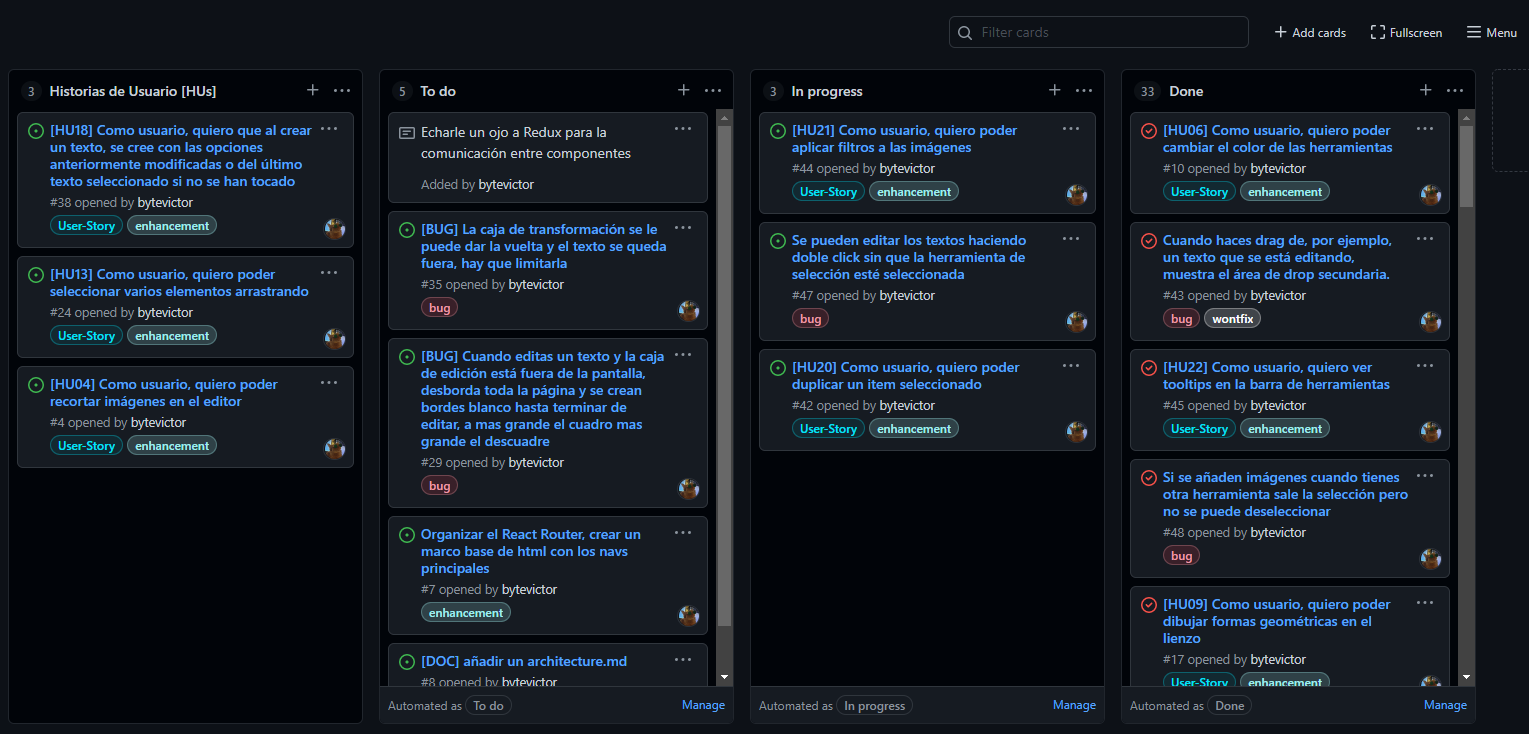
\includegraphics[scale=0.4]{img/kanban.png}}
  \caption{Tabla Kanban del proyecto de Github de MemeHub.}
\end{figure}